\chapter{绪论}
\label{cha:chap1}
\section{研究背景和研究意义}
\label{sec:1.1}
\subsection{研究背景}
\label{sec:1.1.1}
人类通过双眼来探索与发现世界,在接收外部信息的方式中,有不到三成来自于听觉、触觉、嗅觉等感受器官,而超过七成、最丰富、最复杂
的信息则通过视觉进行感知的。计算机视觉便是一种探索给计算机装备眼睛(摄像头)与大脑(算法)的技术,以使计算机能够自主独立的控
制行为、解决问题,同时感知、理解、分析外部环境。

20世纪60年代,计算机视觉得到了最初的发展,该阶段的研究重心主要体现在如何从二维图像中恢复出如立方体、圆柱体等立体化的三维形
状,解释各个物体的空间位置关系。1982年David Marr从信息处理的角度对数学、神经生理学、计算机图形学等学科的研究成果进行了归纳
总结,并在此基础上提出了一系列计算机视觉理论,经典Marr视觉信息处理过程如图~\ref{fig:introduction_Marr}所示。得益于这个完
整明确的理论体系,计算机视觉得到了蓬勃的发展,它的核心思想是从二维图像恢复三维结构。
\begin{figure}[H] % use float package if you want it here
  \centering
  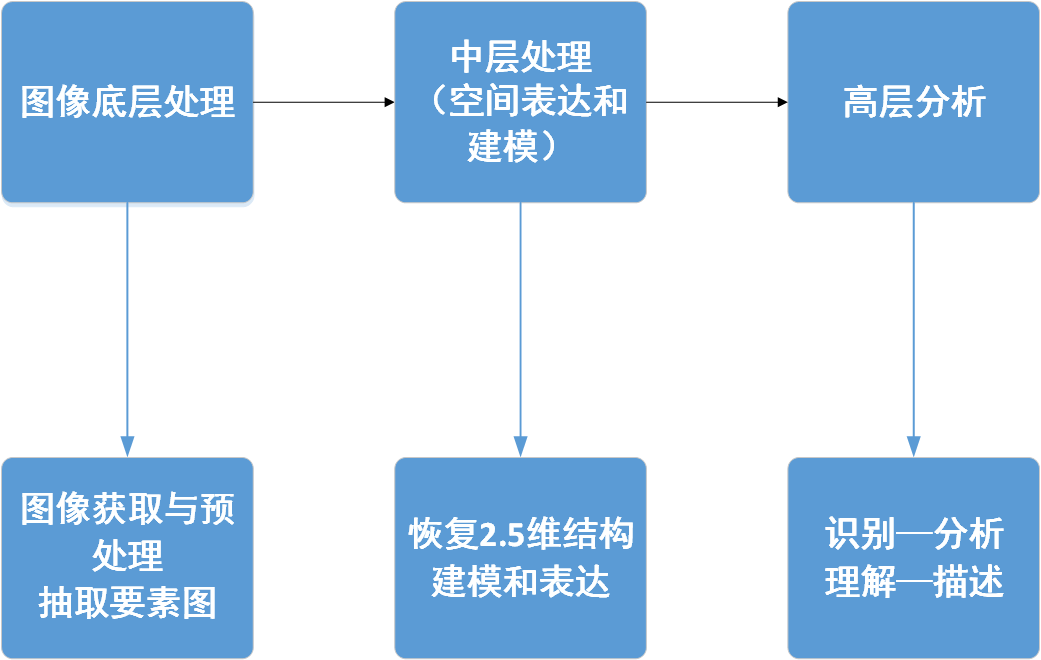
\includegraphics[height=6cm]{introduction_Marr.png}
  \caption{经典Marr视觉信息处理过程示意图}
  \label{fig:introduction_Marr}
\end{figure}
近年来,图像的三维重建在计算机视觉中发挥了很大的作用,并且在质量和性能上有了较大的提升。其主要应用是自动地对于难以建模的对象
建模,加快了图像运用的建模过程。这种技术需要处理大量的数据,可以使用于室内和室外的场景, 而不受控制的环境通常影响室外场景,如
密集建筑群,或者复杂的原始森林等。对于这些场景,虚拟现实和计算机模拟可以被用来分析工作环境和工作难度等方面,三维图像重建技术
本身被视为一个生成3D模型的技术。快速有效完整重建类似于雕塑三维物体目标的三维模型成为目前的研究方向。由连续图像的三维重建主要
是指从二维图像序列中的获取物体的信息并进行三维重建。然而,这个领域并没有引起人们足够的重视,因此本文将对三维重建的具体原理以及
改善展开讨论。

当前在一些工业场景中,需要对其中场景进行测量,主要包括场景的高度,面积,体积,甚至于温度,湿度分布等,传统方式中主要采用雷
达扫描场景的方式来进行,但考虑到该雷达本身成本较高,受场景的限制也很大,在室外环境或者大尺度环境下,就难以发挥作用。现在更多
采用计算机视觉的方式来解决这些问题,可以根据三维重建的点云结果测量以上所描述的几何特性,这样做只需要结合摄像机和测量算法即
可实现,可以很简易的复现在多种场合中。
\subsection{研究意义}
\label{sec:1.1.2}
本文的研究目标是让无人机能够在全封闭或者半封闭的环境中,完全基于视觉的方法完成自主飞行任务,并且在飞行的过程中,采集待测物
体的实拍图像,进行三维重建,最终根据三维重建的点云结果测算待测物体的体积值。

传统无人机的飞行都需要依靠操作员手动控制,或者是基于GPS定位结果进行巡航,本文提出了一种完全基于纯视觉的方法来进行无人机定位
的导航得到的方法,该方法可以在全封闭无GPS的环境中,为无人机提供定位信息,解决了场景限制的问题,并且整个无人机的飞行过程可以
完全自动化的运行,并对场景进行图像采集。

从二维图像重建三维立体具有重要的研究价值和潜在经济社会价值,其核心技术是通过运动来恢复结构。三维重建系统在不同的应用领域有
着不同的预设条件和技术要求,主要包括医学领域的重建系统,机器人导航相关实时重建系统,工业领域包括3D打印在内的室内高精度重建
系统,以及摄影测量领域实景三维重建系统。 三维重建已能提供完整方案,但传统三维重建算法得到的点云结果存在精确度不高,场景无
法闭合等问题,本文提出一种结合SLAM结果的三维重建方法,拟生成一个高精度,强鲁棒的点云地图。

有关实景物体三维测量,传统方法常采用激光雷达,声波等方案,这些方案成本较高,且对场景有限制要求要求,本文提出了一种基于三维
重建后的点云结果进行体积估计的方法,可以极大降低成本且能够在多重场合下复用算法。

因此基于无人机自主飞行采集图像数据的三维重建和体积测量有着十分重要的工程意义,并且在很多场合下,整体流程可靠性和可行性都得
到充分验证。


\section{国内外研究现状}
\label{sec:1.2}
基于
\subsection{SLAM的研究现状}
\label{sec:1.2.1}
SLAM(即时建图与定位)是一种在定位导航的同时,进行构图的技术\cite{cadena2016past}。最早的SLAM技术还不是使用视觉的方法,
而是使用声波传感器或者激光以及惯性测量单元实现环境建模和自身定位,直到21世纪,Stephen Se等人首次使用图像的特征点实现视觉
SLAM\cite{se2002mobile},之后由$Davison$使用$EKF$框架实现了最早的单目实时SLAM系统\cite{davison2003real},奠定了单目系统
的基础;Davison在2007年成功实现基于单相机的纯视觉SLAM系统,算法的关键是在线建立2D点到3D点的映射关系,并且使用实时运动模
型估计相机的位置\cite{davison2007monoslam};Mur-Artal使用ORB特征点作为地图构建特征点,大幅度降低了点云的数量,并且使用
回环检测的方法使定位与建图的精度都大幅提升\cite{mur2015orb};随着硬件计算能力和数据储存的提升,提取目标深度信息的技术得
到了很大的发展,戚传江等人使用2D slam的解决方案,采用多传感器数据融合的方法,完成多自由度位姿检测,拓展了SLAM的应用场
景;Whelan的实验通过使用体积融合的方法实现了实时大范围的稠密RGB-D的SLAM系统\cite{whelan2015real}。

Durrant-Whyte和Bailey首先对前20年里SLAM的发展做出了详细的历史回顾,
并提出了概率方法和数据融合\cite{Gibbens2000A,durrant2006simultaneous},Aulinas等人提出在SLAM中添加滤波方法减少噪音影响
\cite{cadena2016past},Grisetti等人就SLAM后端进行详细阐述\cite{grisetti2010tutorial},Dissanayake研究了SLAM的基本性质,
包括可观测性、收敛性和一致性等\cite{dissanayake2011review}。近几年来,SLAM的发展更多的开始和机器人领域相结合, 
Saeedi提出了多协同机器人SLAM解决方案\cite{saeedi2016multiple},Stachniss发布了在SLAM领域机器人开发
手册\cite{stachniss2016simultaneous}。

应用到目标跟踪领域,单纯点云集还是无法满足要求,因此需要将点云数据语义化,Reiger使用关系树的方法实现物体的语义识别
\cite{sarkar2012slam},这项技术对于目标跟踪是很重要的;之后Sarkar在Reiger的研究基础上结合FastSLAM的方法,使得识别速度
更快,鲁棒性更强;Zhang, G等人使用基于线条的SLAM算法\cite{zhang2015building}提高物体识别的准确率,该方法能够对物体的边
沿与轮廓进行稳定的识别。

当使用单目相机运行SLAM算法时,依旧还存在很多的挑战,ORB-SLAM2\cite{mur2017orb}和LDSO\cite{gao2018ldso}
可能是目前单目SLAM中最先进的方法。然而,这些方法还存在很多的局限性,无地图复用,无法纯旋转,场景需丰富等,
并且用于重定位的方法\cite{galvez2012bags}在视点变化、重复模式和随时间变化时的性能有限。另一种估计相机姿态的方法是使用放置
在环境中的人工标记,最近的SPM-SLAM\cite{munoz2019spm}解决了之前描述的一些限制,它使用二维码而不是自然特征,但是也存在场
景中摆放大量二维码的问题。UcoSLAM\cite{munoz2019ucoslam}则提出了一种结合自然点和人造二维码的SLAM运行方法。

\subsection{三维重建的研究现状}
\label{sec:1.2.2}
照相机/摄像机是将一个三维场景或物体投影到二维平面上,但是在降维的过程不可避免地会损失存在信息,而利用三维重建技术,就是从获
取到的二维图像中复原原始三维场景或物体,三维重建的结果如图~\ref{fig:3d_constr}所示。

\begin{figure}[H] % use float package if you want it here
    \centering
    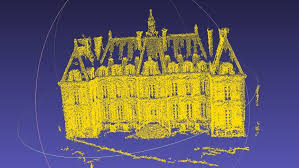
\includegraphics[height=8cm]{3d_constr.png}
    \caption{三维重建结果示意图}
    \label{fig:3d_constr}
  \end{figure}
CMU大学的Tomasi和Kanade\cite{tomasi1992shape}等人首先开发出了基于图片的三维重建系统,并利用仿射分解法对摄像机进行了标定,
得到摄像机运动参数,然后重构出物体的空间模型。随后,INRIAB Bougnoux等人\cite{bougnoux1997totalcalib,debevec1998image}
利用未标定的SfM和摄像机自标定等算法,开发了一个提升型三维重建模型。Berkeley大学的Debevoc\cite{beardsley19963d}等人完成了
著名的建筑物重构系统Façade,该系统要求首先得到建筑物的粗略几何模型和摄像机运动参数。Shum等人开发的人机交互式重构系统,利用
物体的一组全景图,即从各个角度得到物体的n张图片,然后对这些图像进行处理,重构出其三维实体,或者将场景表示成一系列按深度划分
的分层的集合。Faugeras等采用摄像机的自标定方法,利用分层重构等经典的方法,从图像序列中重构出建筑物的形貌。Katholieke大学
的Pollefeys等提出物体表面自动生成系统,该系统是在内参数可以改变的情况下,对摄像机采取了自标定的技术,该系统只要求用摄像机
绕物体周围一周,拍到一系列的图像,就可以自动实现自标定和分层重构。

\subsection{基于视觉体积测算的研究现状}
\label{sec:1.2.3}
基于
\subsection{语义结构化地图的研究现状}
\label{sec:1.2.4}
基于
\section{待解决问题}
\label{sec:1.3}
当前基于无人机自主飞行采集图像数据进行三维重建以及体积测量的方案还存在很多的待解决问题,如:\\
(1)	无人机在完全封闭环境中依靠纯视觉进行定位和建图,难以获取高精度的飞行位姿和地图信息。\\
(2)	基于三维重建算法对场景进行三维重建时,面临整个流程耗时长,输出点云噪音点大,需要对传统三维重建进行提升,以获取高精度
强鲁棒性的大尺度地图。\\
(3)	基于三维点云的体积测算,点云中缺少水平面信息,尺度信息,导致无法直接获取到体积真值。
\section{主要研究内容和技术路线}
\label{sec:1.4}
本文将针对目前无人机在无GPS的密闭环境中进行自主飞行存在的问题,采用计算机视觉的方式建立一套稳定,高精度的无人机自主定位系
统,并对采集到的图像作为输入开发出一套能够生产高精度,强鲁棒的三维重建系统。针对获取到的三维点云,提出估计尺度,确定水平面
的方法以获取感兴趣区域的堆体体积本文将针对上述功能开发出一套完整、全自动化的系统。所研究系统将得到以下指标:\\
1)	建立一套无人机自动定位凶系统,使得无人机自主定位结果与真实GPS定位数值误差在0.5米以内,位置差距在2$\%$之内。\\
2)	建立一套基于视频流,并融合SLAM结果的和高精度三维重建系统,能够针对各种室内外的大尺度建筑物场景实现三维重建,场景场能将
误差控制在20cm以内。\\
3)	建立一套堆体体积自主测量系统,可以快速估计出点云的尺度,水平面方程与堆体体积,测量误差控制在2$\%$之内。\\
4)	建立一套基于无人机自主飞行采集图像数据进行三维重建以及体积测量的完整方案,实现快速全自动的测量流程。

结合研究内容,完成理论研究,系统实现以及测试实验与分析,技术路线如图~\ref{fig:introduction_pipeline}所示。
\begin{figure}[H] % use float package if you want it here
  \centering
  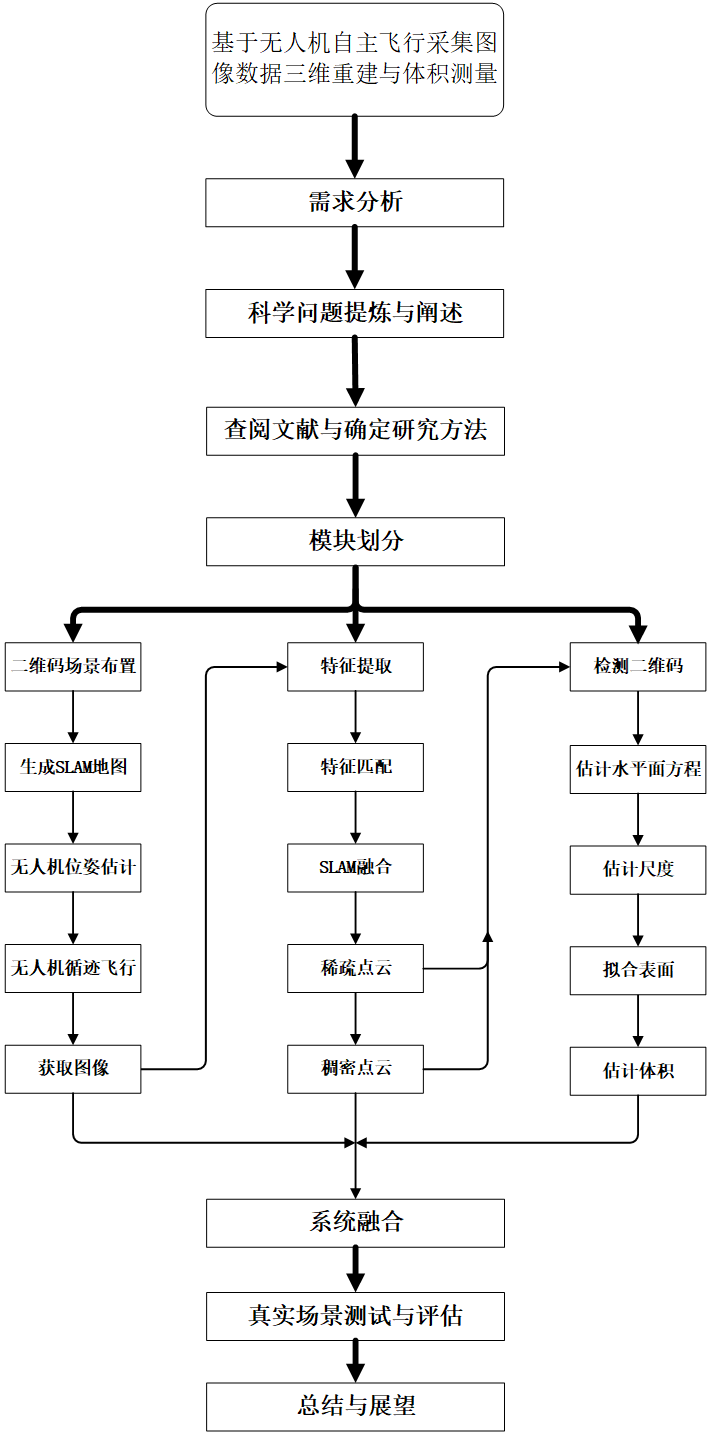
\includegraphics[height=22.5cm]{introduction_pipeline.png}
  \caption{技术路线图}
  \label{fig:introduction_pipeline}
\end{figure}
\section{章节安排}
\label{sec:1.4}

